|\chapter{Instalación}

En este apéndice se mostrará los pasos necesarios para realizar la instalación de la aplicación y sus dependencias

\section{Instalación de la aplicación}
El usuario cuenta con múltiples opciones ya que la aplicación se ha desarrollado empleando Unity, una tecnología multiplataforma, 
sin embargo, se recomienda la instalación en entornos móviles ya que ha sido desarrollada con tal objetivo.

\subsection{Android}
Para instalar la aplicación en Android es necesario previamente configurar el dispositivo para permitir 
la ejecución de programas de terceros o de lo contrario el \textit{smartphone}
la bloqueará ya que no se encuentra desplegada en Google Play.

En dispositivos Android 8.0 o superior se debe conceder permisos de instalación a la aplicación desde 
la que se descargará el fichero APK. Estas opciones comunmente se encuentran en 
\textit{Ajustes>Aplicaciones>Acceso especial a aplicaciones>Instalar aplicaciones desconocidas}.
Se debe seleccionar el navegador empleado para descargar el fichero o la aplicación de la que se vaya 
a obtener.
\begin{figure}[htbp]
    \centering
    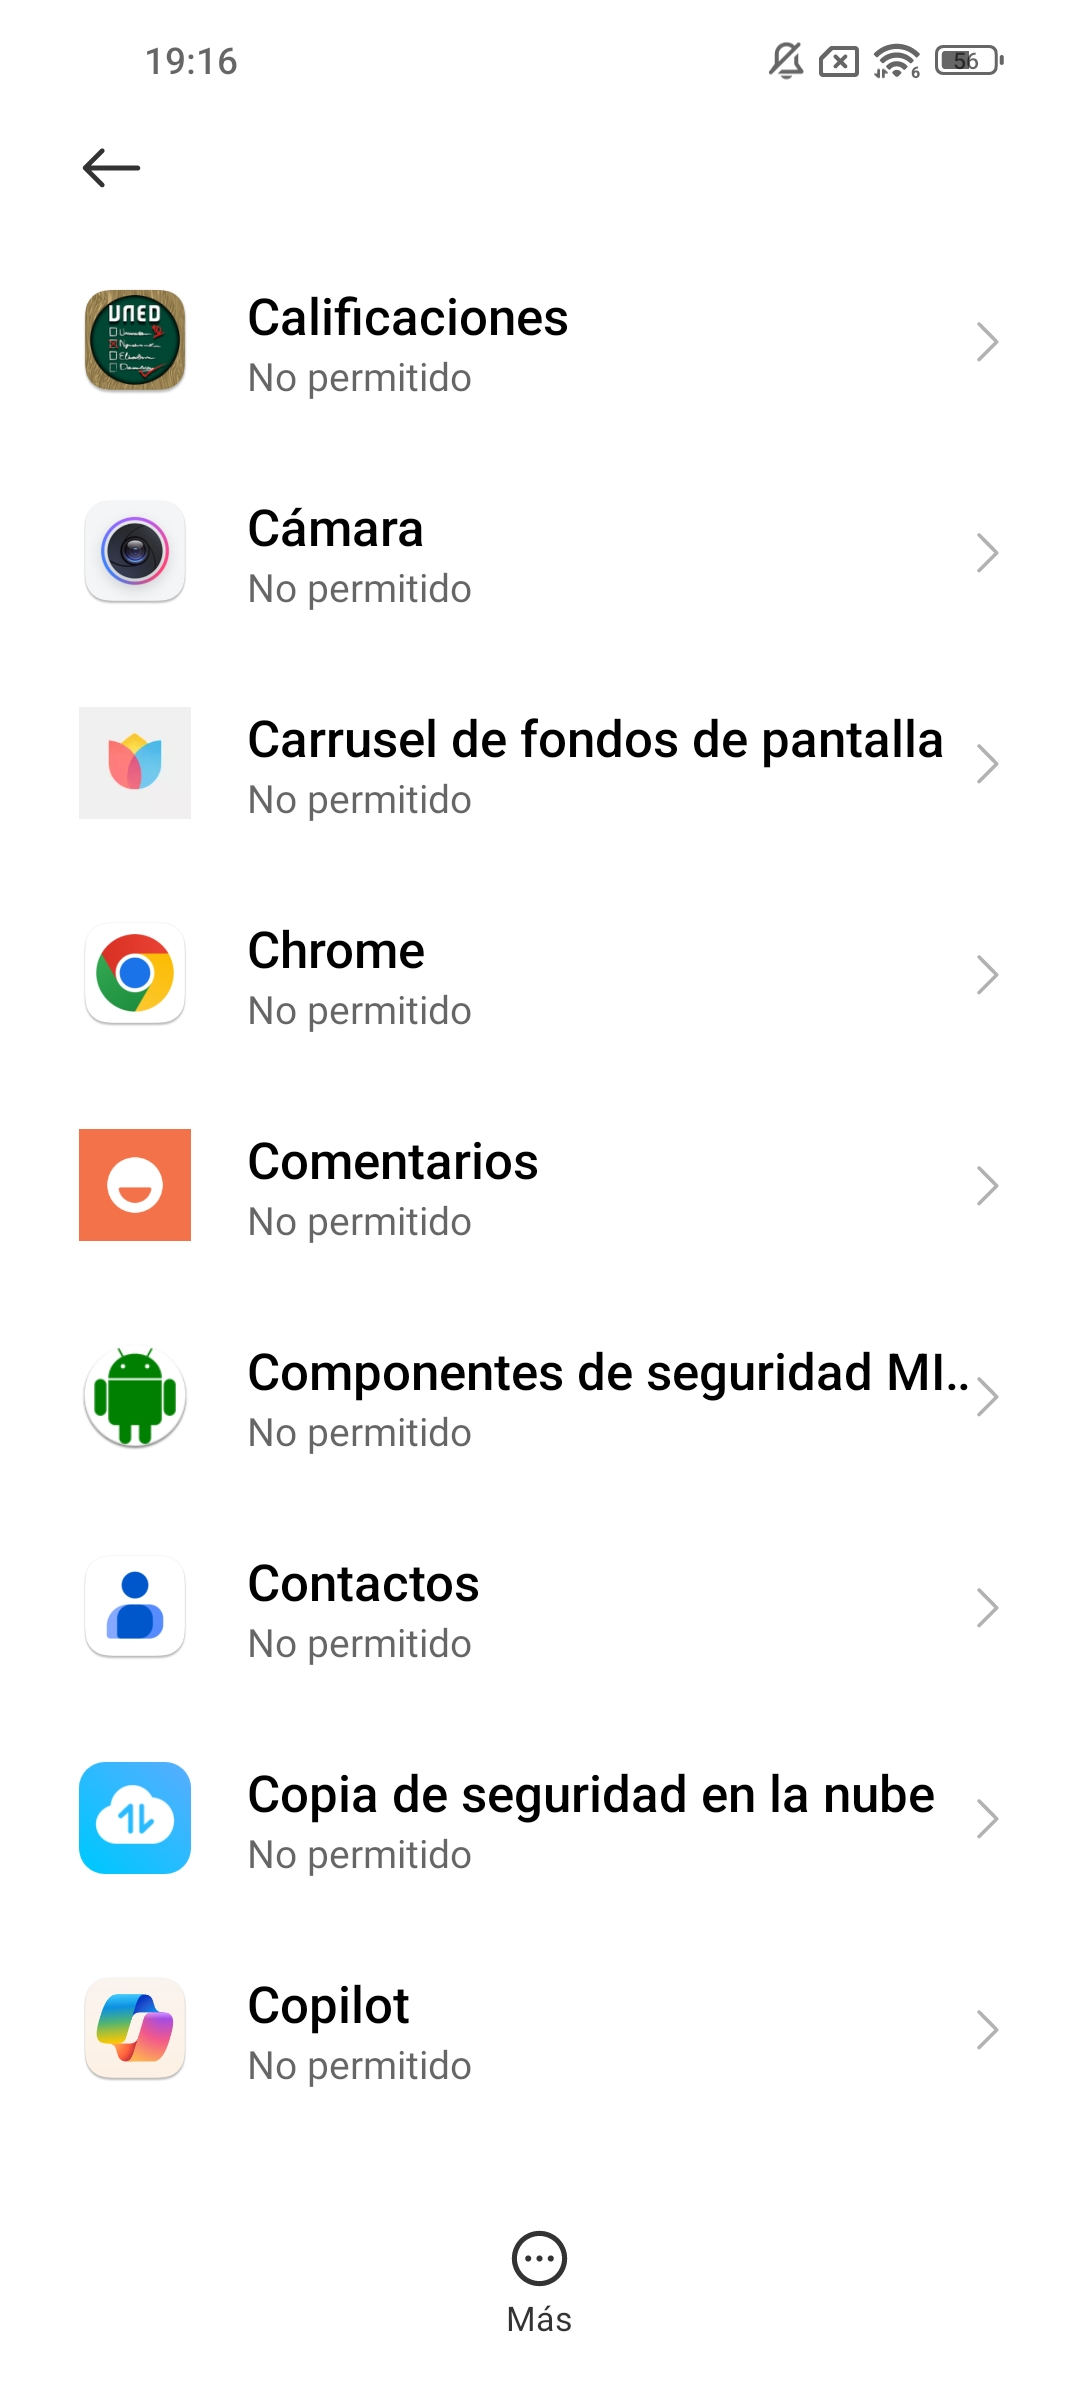
\includegraphics[width=0.8\textwidth]{imagenes/instalacion/apps_desconocidas.jpg}
    \caption{Selección de aplicación fuente de instalacion de aplicaciones desconocidas.}
    \label{fig:allow_install_unkn_apps}
\end{figure}
\begin{figure}[htbp]
    \centering
    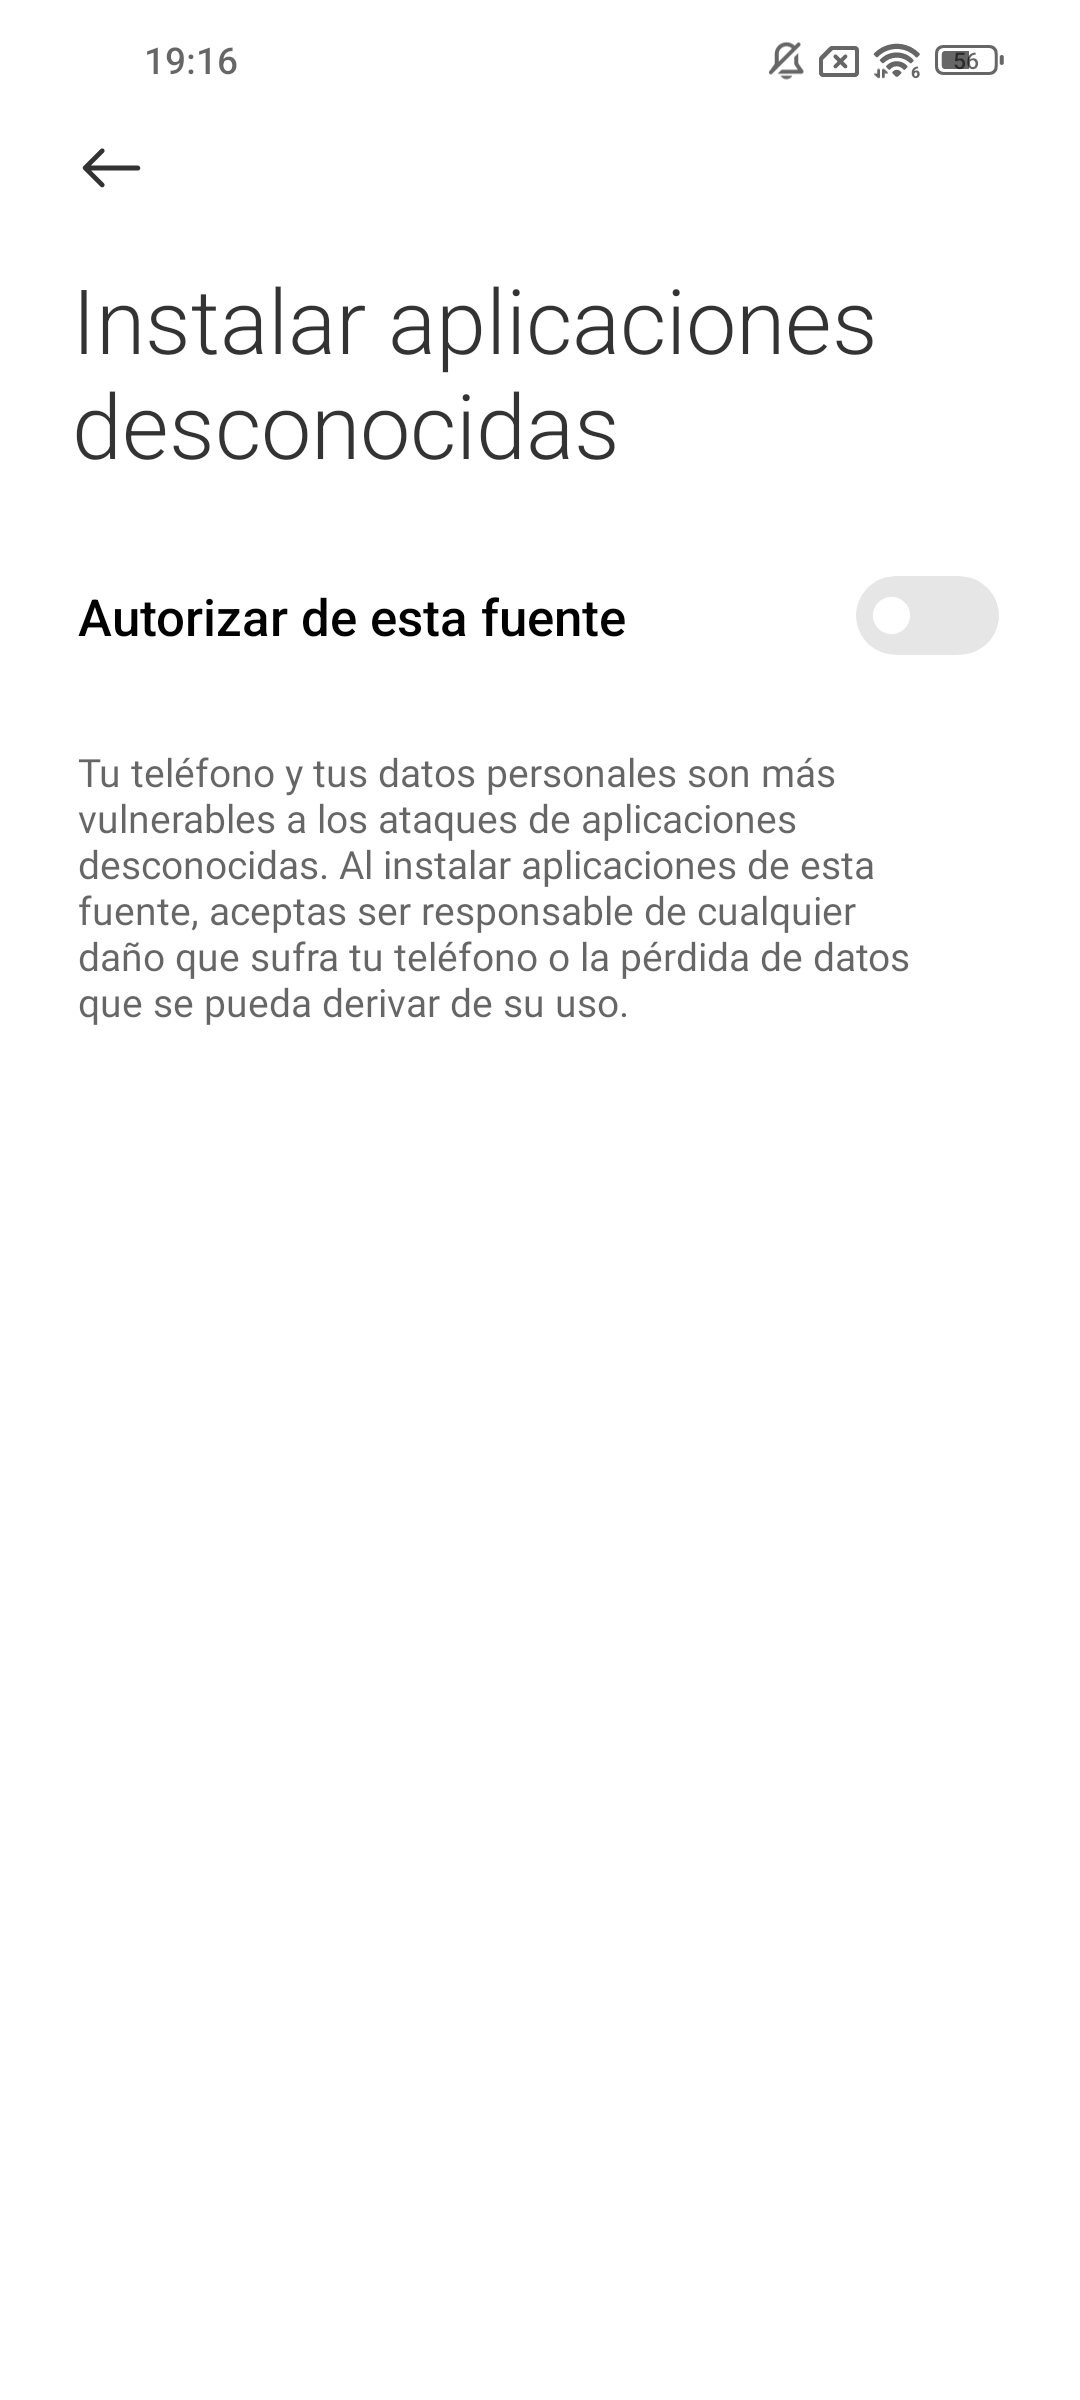
\includegraphics[width=0.8\textwidth]{imagenes/instalacion/autorizar_fuente.jpg}
    \caption{Autorización de aplicación fuente.}
    \label{fig:auth_source}
\end{figure}

Es posible que al intentar autorizar la fuente el teléfono avise sobre los riesgos 
de instalar aplicaciones de terceros. Para instalarla se debe aceptar el riesgo y continuar, pero 
es recomendable volver a denegar los permisos tras la instalación.
\begin{figure}[htbp]
    \centering
    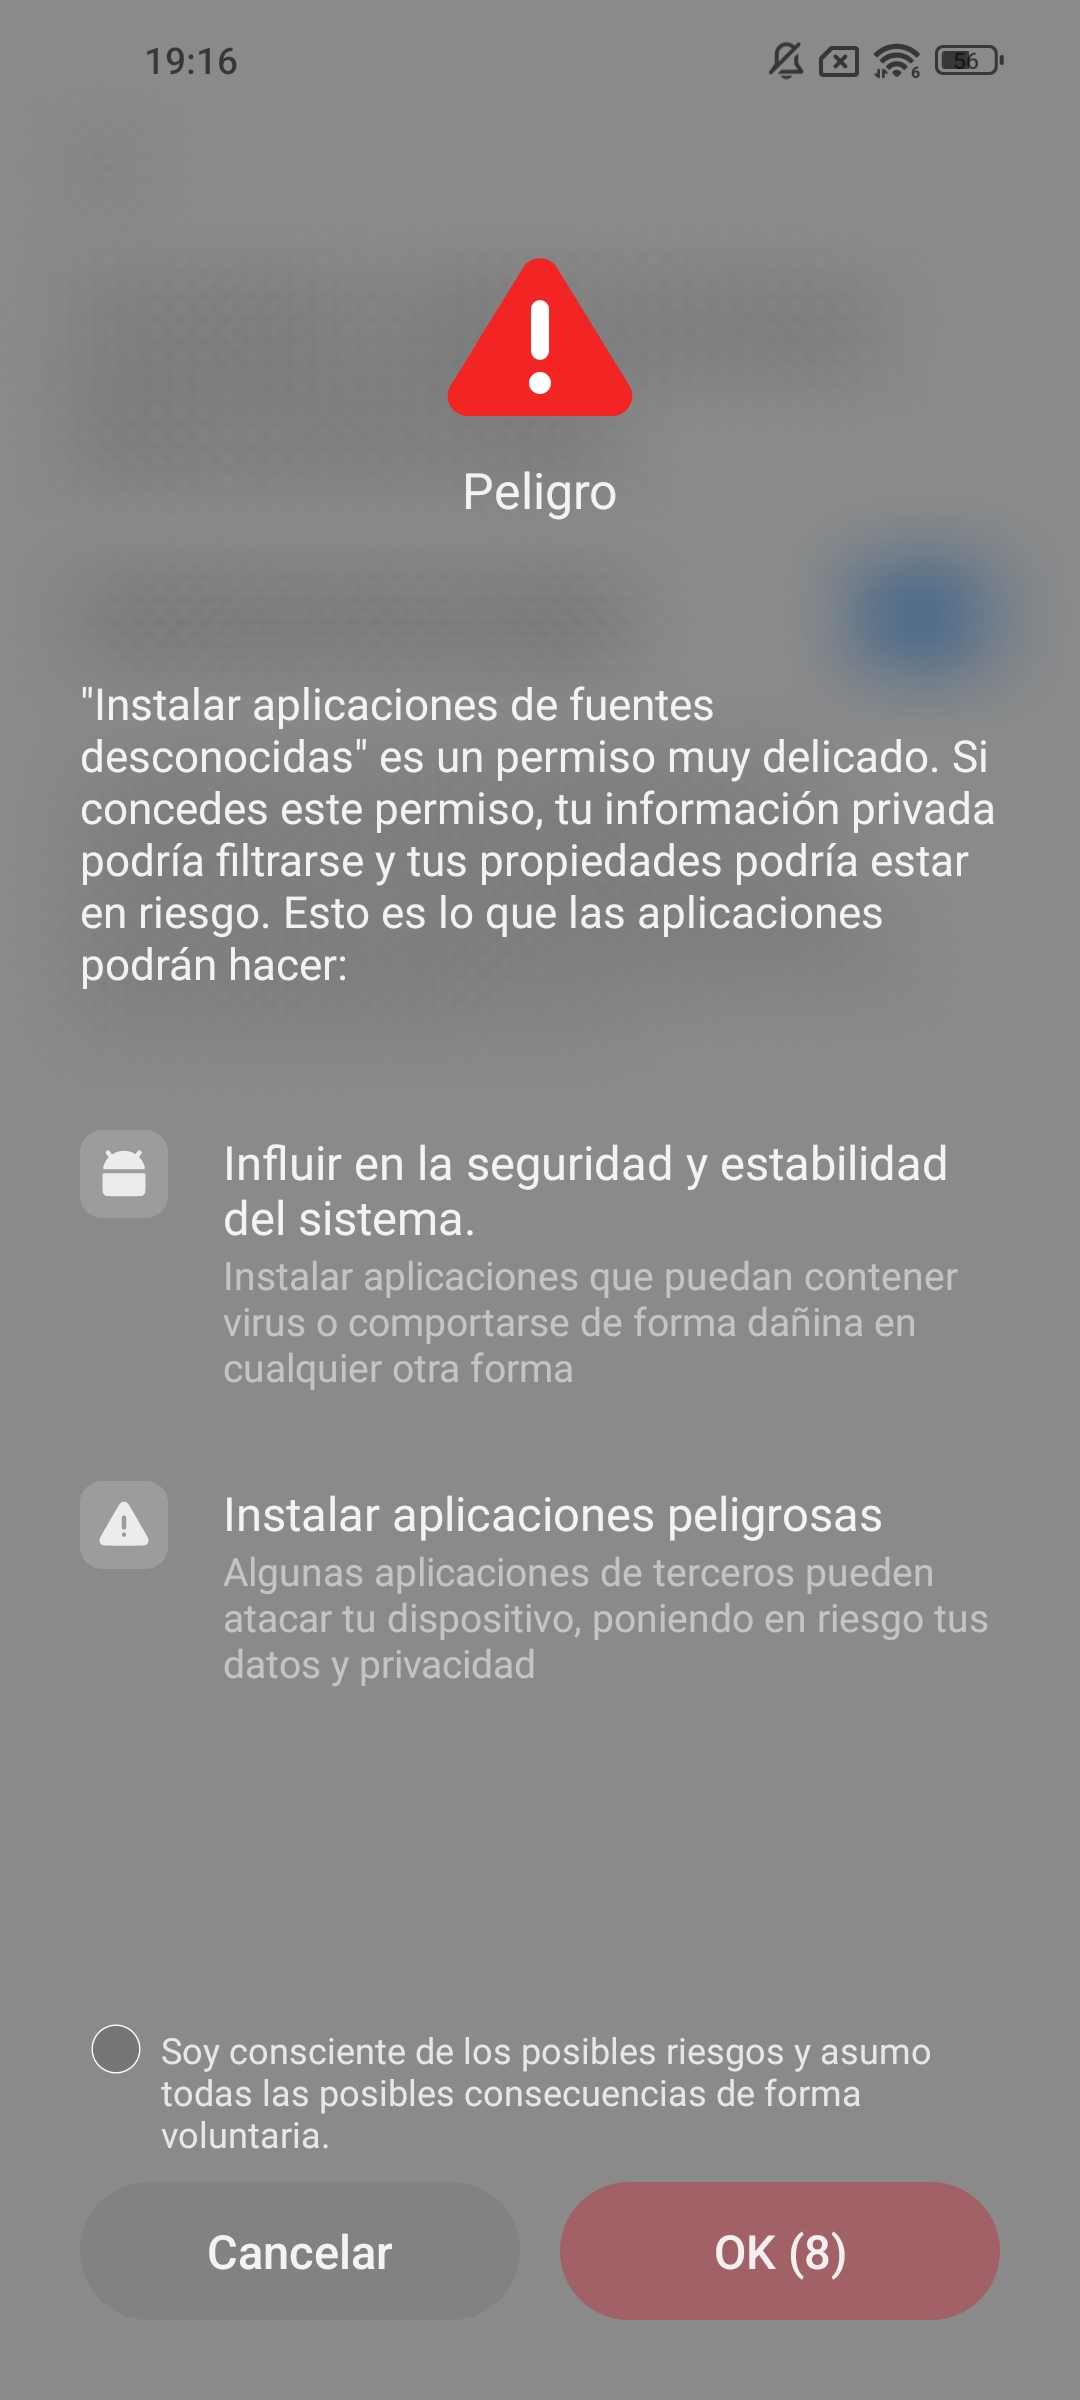
\includegraphics[width=0.8\textwidth]{imagenes/instalacion/aviso.jpg}
    \caption{Aviso de riesgos en instalación de aplicaciones de terceros.}
    \label{fig:warning}
\end{figure}

Una vez aceptado comenzará el proceso de instalacion.
\begin{figure}[htbp]
    \centering
    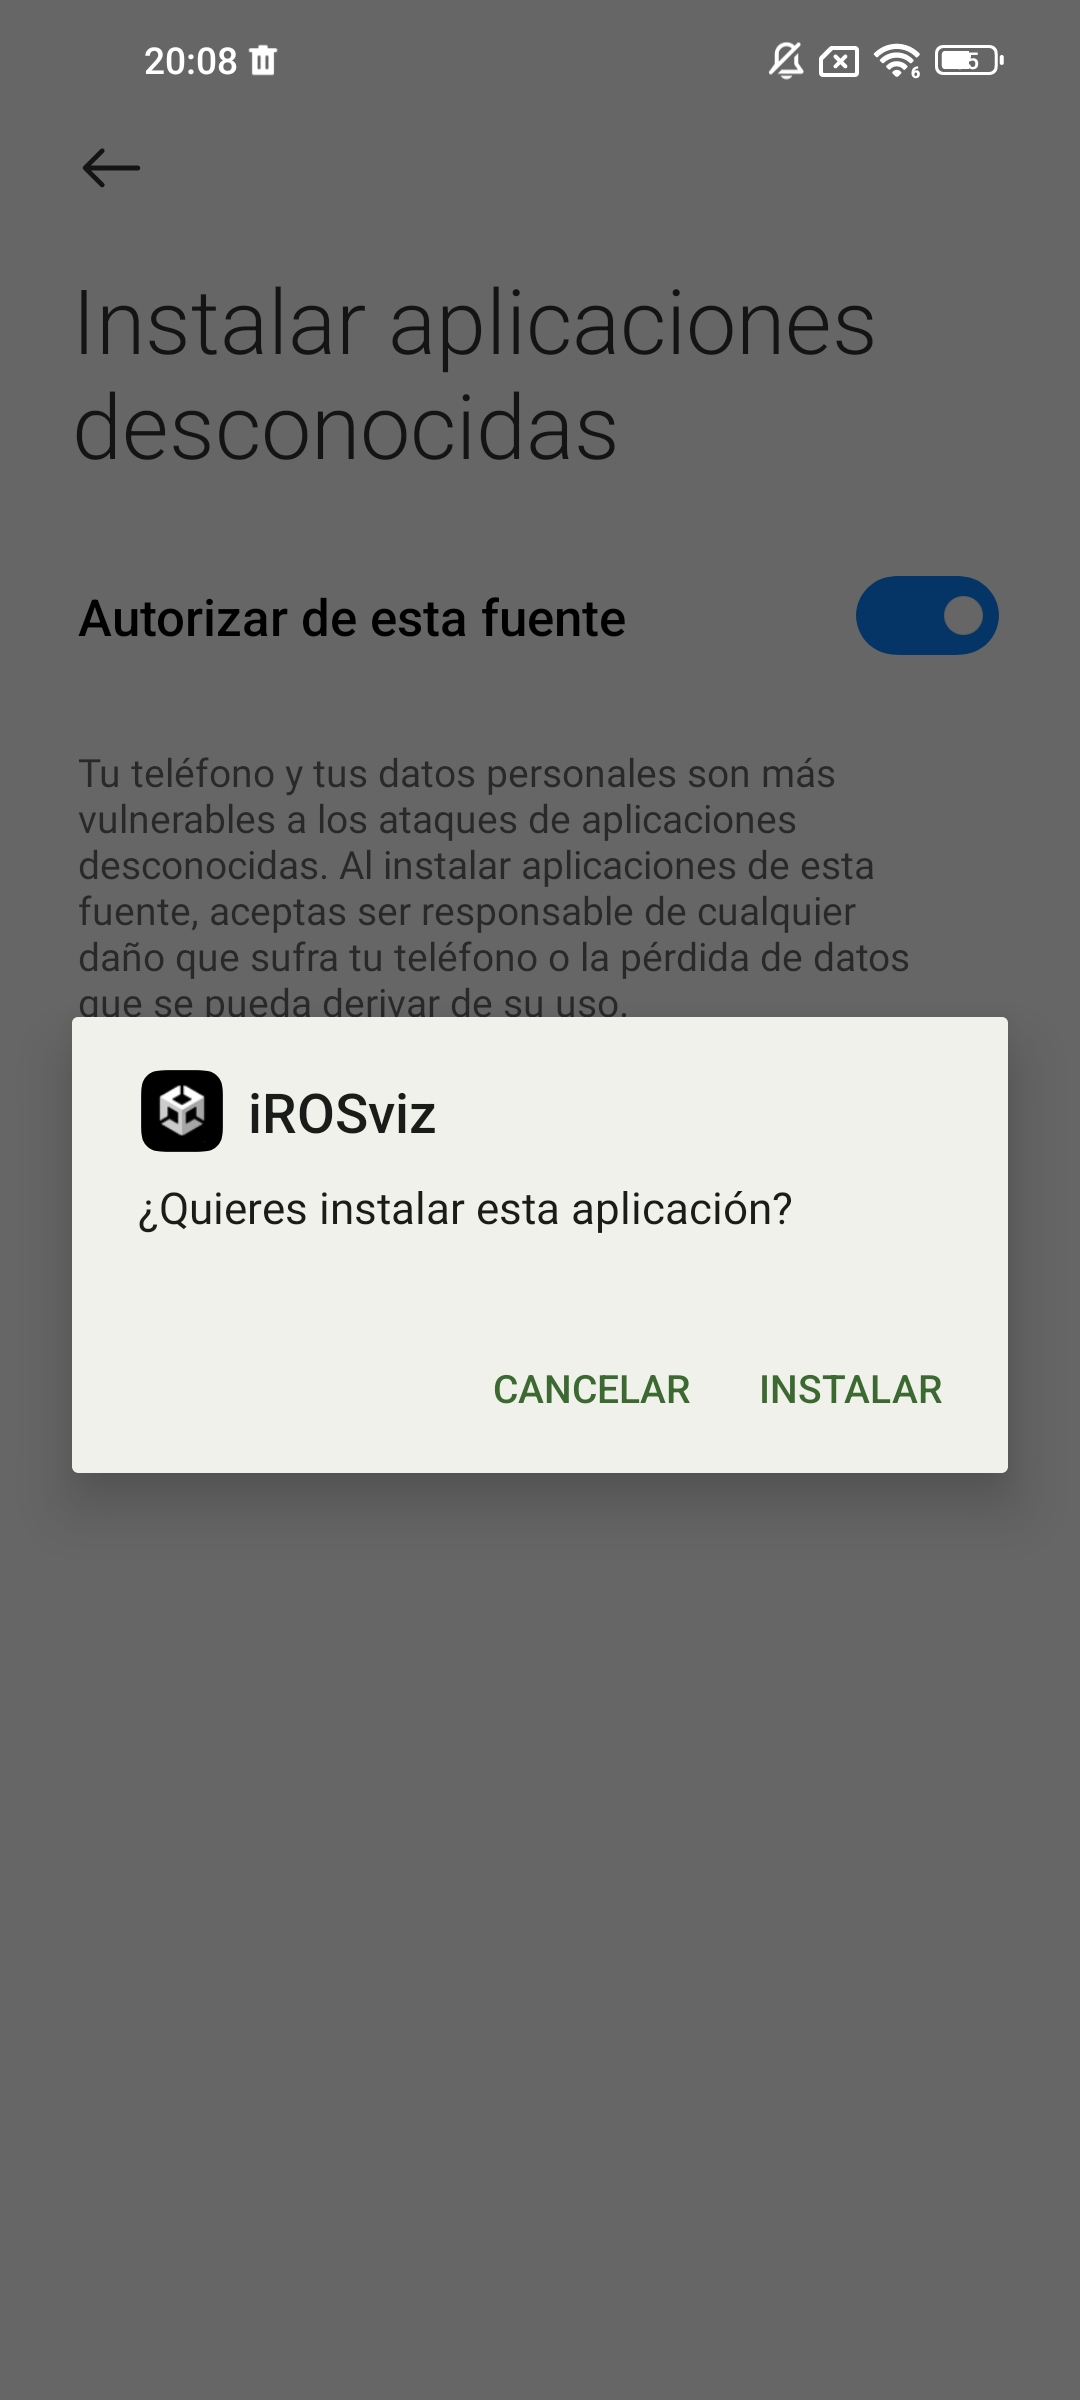
\includegraphics[width=0.8\textwidth]{imagenes/instalacion/instalar_app.jpg}
    \caption{Instalación aplicación.}
    \label{fig:install_app}
\end{figure}

\subsection{Linux}
Para instalar la aplicación en Linux es necesario descomprimir el directorio \textit{iRozViz_linux.zip} 
haciendo clic derecho y seleccionando "Extract here" en caso de que el sistema operativo cuente con herramientas
de compresión de ficheros o se haya instalado una específica.
\begin{figure}[htbp]
    \centering
    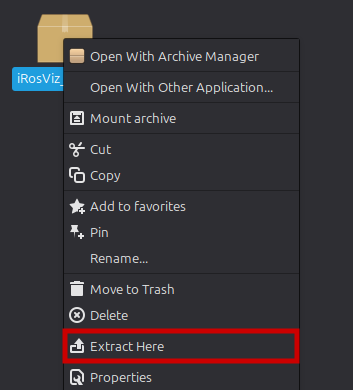
\includegraphics[width=0.8\textwidth]{imagenes/instalacion/dialog_extract_linux.png}
    \caption{Cuadro diálogo extracción comprimido. Linux.}
    \label{fig:dialog_extract_zip_linux}
\end{figure}

Para inicar la aplicación ahora solo es necesario ejecutar el fichero \textit{iRosViz.x86_64} dentro del directorio generado.

\subsection{Windows}
Dependiendo de la arquitectura sobre la que se ejecute el sistema operativo, se debe descargar una opción u otra.

Si se dispone de una máquina con arquitectura ARM se debe descargar el comprimido \textit{iRosViz_windows_arm_64.zip}.
De lo contrario, si se dispone de una máquina x86_64 se debe descargar el comprimido \textit{iRosViz_windows_x86_64.zip}.

Una vez descargado el documento, se puede alojar en cualquier carpeta deseada y descomprimirlo empleando cualquier
herramienta de gestión de ficheros comprimidos.
Puesto que las últimas versiones de Windows incluyen esta herramienta
de manera nativa, se realizará la explicación con ellas.

Haciendo clic derecho en el comprimido, se debe seleccionar la opción "Extraer todo...". 
\begin{figure}[htbp]
    \centering
    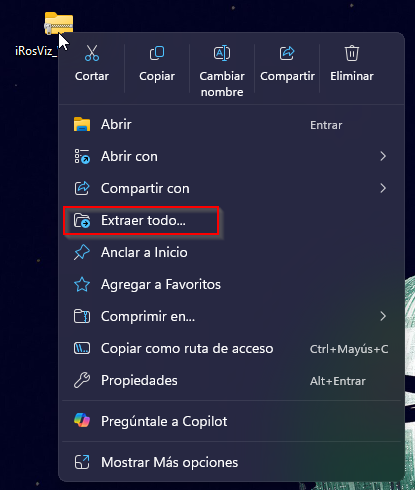
\includegraphics[width=0.8\textwidth]{imagenes/instalacion/dialog_extraer.png}
    \caption{Cuadro diálogo extracción comprimido. Windows.}
    \label{fig:dialog_extract_zip}
\end{figure}

La herramienta solicitará
una ruta sobre la que extraer los ficheros que podrá ser modificada a voluntad del usuario.
\begin{figure}[htbp]
    \centering
    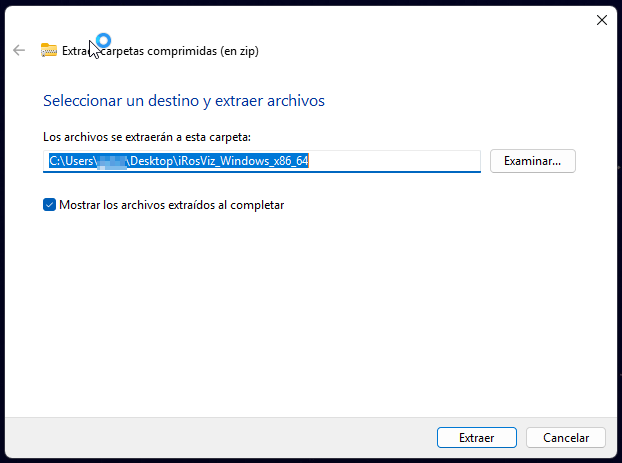
\includegraphics[width=0.8\textwidth]{imagenes/instalacion/dialog_extraer_fichero.png}
    \caption{Ventana extracción comprimido}
    \label{fig:extract_zip_window}
\end{figure}

Una vez se hace clic en "Extraer..." comienza el proceso y tras finalizar ya se tiene acceso a la carpeta descomprimida.
\begin{figure}[htbp]
    \centering
    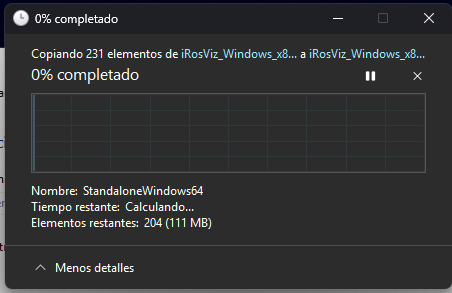
\includegraphics[width=0.8\textwidth]{imagenes/instalacion/ficheros_extaryendo.png}
    \caption{Extracción ficheros}
    \label{fig:files_extract}
\end{figure}

\section{Instalación de ROS en servidor}
La distribución recomendada de ROS2 es \textbf{Jazzy Jalisco}, de hecho, es con la que se ha realizado el desarrollo
y que garantiza que todas las funcionalidades funcionen correctamente. Sin embargo, pueden 
instalarse distribuciones diferentes siempre y cuando se traten de ROS2 y versiones superiores a la mencionada.

En cuanto al sistema operativo, ROS2 Jazzy Jalisco indica en su documentación que debe ejecutarse sobre distribuciones 
\textbf{Ubuntu 24.04}. A pesar de esto, el desarrollo se ha realizado con Linux Mint 22.2 sin problemáticas.

La guía de instalación está dispobible en la 
\href{https://docs.ros.org/en/jazzy/Installation/Ubuntu-Install-Debs.html}{página web oficial de la documentación de ROS}

\section{Ejecución del servicio en el servidor}
El servicio ROS es el puente de comunicación entre la aplicación y el entorno ROS donde se encuentra toda la lógica robótica.
Como se ha comentado en secciones anteriores, se realizaron diversos intentos de incluir la distribución de ROS como 
\textit{plug-in} nativo en la propia aplicación, pero no fue posible por problemas de compilación cruzada.

Para iniciar el servicio se debe instalar previamente la versión de ROS indicada, descargar el 
espacio de trabajo ROS \textit{ros2_ws} y ejecutar el \textit{script startup.sh}.
Este añadirá las fuentes necesarias de la conexión ROS mediante TCP y los servicios necesarios.
